% answers.tex —— 1999 年·全国卷·理科 · 参考答案与详细解析片段
% 由 tools/generate_projects.py 依来源总账自 1999/1999_数学真题_全国理_试题.md + 1999/1999_数学真题_全国理_解析正文.md + 1999/1999_数学真题_全国理_答案要点.md 生成，勿手改（改源 MD 后重跑）


\begin{gktip}
固定源 PDF 只有一页题面，没有答案和解析页。以下各题均依据题面独立复算；第 1、10、21、22、24 题的图形在 LaTeX 工程中以 TikZ/PGFPlots 矢量源重绘。
\end{gktip}

\begin{answer}
\gksolhead{1}{}

\textbf{题目}：

如图，$I$ 是全集，$M$、$P$、$S$ 是 $I$ 的 3 个子集，则阴影部分所表示的集合是\mbox{（　　）}
\nopagebreak[4]
\begin{center}% 1999 年全国卷理科第 1 题：集合关系图
% 仅保留 TikZ 矢量源；阴影表示 (M \cap P) \cap \overline S。
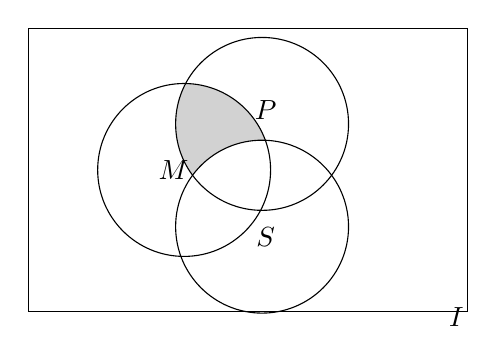
\begin{tikzpicture}[scale=0.9]
  \coordinate (M) at (2.2,2.0);
  \coordinate (P) at (3.3,2.65);
  \coordinate (S) at (3.3,1.2);

  \draw (0,0) rectangle (6.2,4.0);
  \begin{scope}
    \clip (M) circle (1.22);
    \clip (P) circle (1.22);
    \fill[gray!35] (0,0) rectangle (6.2,4.0);
  \end{scope}
  % Erase the part inside S, then redraw all boundaries on top.
  \fill[white] (S) circle (1.22);
  \draw (0,0) rectangle (6.2,4.0);
  \draw (M) circle (1.22);
  \draw (P) circle (1.22);
  \draw (S) circle (1.22);

  \node at (2.05,2.0) {$M$};
  \node at (3.35,2.85) {$P$};
  \node at (3.35,1.05) {$S$};
  \node[below right] at (5.8,0.2) {$I$};
\end{tikzpicture}
\end{center}
\nopagebreak[4]
（A）$(M\cap P)\cap S$　　（B）$(M\cap P)\cup S$

（C）$(M\cap P)\cap\overline S$　　（D）$(M\cap P)\cup\overline S$

\Needspace{4\baselineskip}
\textbf{解析}

\Needspace{5\baselineskip}
由图可见，阴影区域同时属于 $M$ 和 $P$，但不属于 $S$，所以所表示的集合为

\nopagebreak[4]
\[
(M\cap P)\cap\overline S.
\]

因此选 C。

\gkanswer{答案：C}

\end{answer}
\begin{answer}
\gksolhead{2}{}

\textbf{题目}：

已知映射 $f:A\to B$，其中，集合 $A=\{-3,-2,-1,1,2,3,4\}$，集合 $B$ 中的元素都是 $A$ 中元素在映射 $f$ 下的象，且对任意的 $a\in A$，在 $B$ 中和它对应的元素是 $|a|$，则集合 $B$ 中元素的个数是\mbox{（　　）}

（A）4　　（B）5　　（C）6　　（D）7

\Needspace{4\baselineskip}
\textbf{解析}

\Needspace{5\baselineskip}
映射的对应关系为 $a\mapsto|a|$。集合 $A$ 中的元素的绝对值只有

\nopagebreak[4]
\[
1,\ 2,\ 3,\ 4
\]

四种，所以集合 $B$ 有 4 个元素，选 A。

\gkanswer{答案：A}

\end{answer}
\begin{answer}
\gksolhead{3}{}

\textbf{题目}：

若函数 $y=f(x)$ 的反函数是 $y=g(x)$，$f(a)=b$，$ab\ne0$，则 $g(b)$ 等于\mbox{（　　）}

（A）$a$　　（B）$a^{-1}$　　（C）$b$　　（D）$b^{-1}$

\Needspace{4\baselineskip}
\textbf{解析}

\Needspace{5\baselineskip}
反函数的定义给出

\nopagebreak[4]
\[
f(a)=b\Longleftrightarrow g(b)=a.
\]

所以选 A。

\gkanswer{答案：A}

\end{answer}
\begin{answer}
\gksolhead{4}{}

\textbf{题目}：

函数 $f(x)=M\sin(\omega x+\varphi)\ (\omega>0)$ 在区间 $[a,b]$ 上是增函数，且 $f(a)=-M$，$f(b)=M$，则函数 $g(x)=M\cos(\omega x+\varphi)$ 在 $[a,b]$ 上\mbox{（　　）}

（A）是增函数　　（B）是减函数

（C）可以取得最大值 $M$　　（D）可以取得最小值 $-M$

\Needspace{4\baselineskip}
\textbf{解析}

\Needspace{5\baselineskip}
令

\nopagebreak[4]
\[
\omega x+\varphi=t.
\]

\Needspace{5\baselineskip}
因为 $f(x)=M\sin t$ 在 $[a,b]$ 上递增，并且端点值从 $-M$ 变到 $M$，所以相应的 $t$ 区间从

\nopagebreak[4]
\[
-\frac\pi2+2k\pi
\quad\text{\text{变到}}\quad
\frac\pi2+2k\pi
\]

\Needspace{5\baselineskip}
其中 $k$ 为整数。该区间包含 $t=2k\pi$，故

\nopagebreak[4]
\[
g(x)=M\cos t
\]

可以取得最大值 $M$。因此选 C。

\gkanswer{答案：C}

\end{answer}
\begin{answer}
\gksolhead{5}{}

\textbf{题目}：

若 $f(x)\sin x$ 是周期为 $\pi$ 的奇函数，则 $f(x)$ 可以是\mbox{（　　）}

（A）$\sin x$　　（B）$\cos x$　　（C）$\sin2x$　　（D）$\cos2x$

\Needspace{4\baselineskip}
\textbf{解析}

\Needspace{5\baselineskip}
逐项考察：

\nopagebreak[4]
\[
\sin x\cdot\sin x=\sin^2x
\]

\Needspace{5\baselineskip}
是偶函数；而

\nopagebreak[4]
\[
\cos x\cdot\sin x=\frac12\sin2x
\]

\Needspace{5\baselineskip}
是周期为 $\pi$ 的奇函数。又

\nopagebreak[4]
\[
\sin2x\cdot\sin x
\]

为偶函数，$\cos2x\cdot\sin x$ 不是以 $\pi$ 为周期。因此 $f(x)$ 可以是 $\cos x$，选 B。

\gkanswer{答案：B}

\end{answer}
\begin{answer}
\gksolhead{6}{}

\textbf{题目}：

在极坐标系中，曲线 $\rho=4\sin\left(\theta-\dfrac\pi3\right)$ 关于\mbox{（　　）}

（A）直线 $\theta=\dfrac\pi3$ 轴对称　　（B）直线 $\theta=\dfrac{5\pi}6$ 轴对称

（C）点 $\left(2,\dfrac\pi3\right)$ 中心对称　　（D）极点中心对称

\Needspace{4\baselineskip}
\textbf{解析}

\Needspace{5\baselineskip}
将极坐标方程写成

\nopagebreak[4]
\[
\rho=4\sin\left(\theta-\frac\pi3\right)
=4\cos\left(\theta-\frac{5\pi}6\right).
\]

\Needspace{5\baselineskip}
这是圆心在极坐标 $\left(2,\dfrac{5\pi}6\right)$、半径为 $2$ 的圆。因此它关于过圆心的直线

\nopagebreak[4]
\[
\theta=\frac{5\pi}6
\]

轴对称，选 B。

\gkanswer{答案：B}

\end{answer}
\begin{answer}
\gksolhead{7}{}

\textbf{题目}：

将若干毫升水倒入底面半径为 $2\ \mathrm{cm}$ 的圆柱形器皿中，量得水面的高度为 $6\ \mathrm{cm}$，若将这些水倒入轴截面是正三角形的倒圆锥形器皿中，则水面的高度是\mbox{（　　）}

（A）$6\sqrt3\ \mathrm{cm}$　　（B）$6\ \mathrm{cm}$　　（C）$2\sqrt[3]{18}\ \mathrm{cm}$　　（D）$3\sqrt[3]{12}\ \mathrm{cm}$

\Needspace{4\baselineskip}
\textbf{解析}

\Needspace{5\baselineskip}
圆柱中水的体积为

\nopagebreak[4]
\[
V=\pi\cdot2^2\cdot6=24\pi\ \mathrm{cm^3}.
\]

\Needspace{5\baselineskip}
设倒圆锥水面的高度为 $h$，圆锥底面半径为 $r$。轴截面为正三角形，所以 $h=\sqrt3r$。在高度 $h$ 处的水面半径为

\nopagebreak[4]
\[
\frac r h h=\frac h{\sqrt3}.
\]

\Needspace{5\baselineskip}
因而水的体积为

\nopagebreak[4]
\[
\frac13\pi\left(\frac h{\sqrt3}\right)^2h
=\frac{\pi h^3}{9}.
\]

令其等于 $24\pi$，得 $h^3=216$，即 $h=6\ \mathrm{cm}$。选 B。

\gkanswer{答案：B}

\end{answer}
\begin{answer}
\gksolhead{8}{}

\textbf{题目}：

若 $(2x+\sqrt3)^4=a_0+a_1x+a_2x^2+a_3x^3+a_4x^4$，则 $(a_0+a_2+a_4)^2-(a_1+a_3)^2$ 的值为\mbox{（　　）}

（A）1　　（B）$-1$　　（C）0　　（D）2

\Needspace{4\baselineskip}
\textbf{解析}

\Needspace{5\baselineskip}
记

\nopagebreak[4]
\[
P(x)=(2x+\sqrt3)^4.
\]

\Needspace{5\baselineskip}
则偶次项系数和与奇次项系数和分别为

\nopagebreak[4]
\[
E=a_0+a_2+a_4=\frac{P(1)+P(-1)}2,
\qquad
O=a_1+a_3=\frac{P(1)-P(-1)}2.
\]

\Needspace{5\baselineskip}
所以

\nopagebreak[4]
\[
E^2-O^2=P(1)P(-1)
=(2+\sqrt3)^4(\sqrt3-2)^4
=\bigl((2+\sqrt3)(\sqrt3-2)\bigr)^4=1.
\]

选 A。

\gkanswer{答案：A}

\end{answer}
\begin{answer}
\gksolhead{9}{}

\textbf{题目}：

直线 $\sqrt3x+y-2\sqrt3=0$ 截圆 $x^2+y^2=4$ 得的劣弧所对的圆心角为\mbox{（　　）}

（A）$\dfrac\pi6$　　（B）$\dfrac\pi4$　　（C）$\dfrac\pi3$　　（D）$\dfrac\pi2$

\Needspace{4\baselineskip}
\textbf{解析}

\Needspace{5\baselineskip}
圆心为原点，圆半径为 $2$。圆心到直线

\nopagebreak[4]
\[
\sqrt3x+y-2\sqrt3=0
\]

\Needspace{5\baselineskip}
的距离为

\nopagebreak[4]
\[
d=\frac{2\sqrt3}{\sqrt{3+1}}=\sqrt3.
\]

\Needspace{5\baselineskip}
弦的一半长为

\nopagebreak[4]
\[
\sqrt{2^2-d^2}=1.
\]

\Needspace{5\baselineskip}
设劣弧所对的圆心角为 $\theta$。半弦长为 $1$，半径为 $2$，所以

\nopagebreak[4]
\[
\sin\frac\theta2=\frac12,\qquad \theta=\frac\pi3.
\]

因此选 C。

\gkanswer{答案：C}

\end{answer}
\begin{answer}
\gksolhead{10}{}

\textbf{题目}：

如图，在多面体 $ABCDEF$ 中，已知面 $ABCD$ 是边长为 $3$ 的正方形，$EF\parallel AB$，$EF=\dfrac32$，$EF$ 与面 $ABCD$ 的距离为 $2$，则该多面体的体积为\mbox{（　　）}
\nopagebreak[4]
\begin{center}% 1999 年全国卷理科第 10 题：多面体 ABCDEF
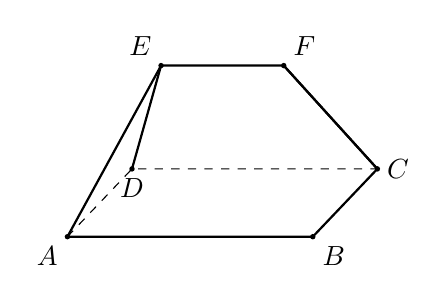
\begin{tikzpicture}[scale=0.82, >=stealth]
  \coordinate (A) at (0,0);
  \coordinate (B) at (3.8,0);
  \coordinate (C) at (4.8,1.05);
  \coordinate (D) at (1.0,1.05);
  \coordinate (E) at (1.45,2.65);
  \coordinate (F) at (3.35,2.65);

  \draw[thick] (A)--(B)--(C)--(F)--(E)--cycle;
  \draw[thick] (F)--(C);
  \draw[dashed] (A)--(D)--(C) (D)--(E);
  \draw[thick] (D)--(E);

  \fill (A) circle (1.2pt) node[below left] {$A$};
  \fill (B) circle (1.2pt) node[below right] {$B$};
  \fill (C) circle (1.2pt) node[right] {$C$};
  \fill (D) circle (1.2pt) node[below] {$D$};
  \fill (E) circle (1.2pt) node[above left] {$E$};
  \fill (F) circle (1.2pt) node[above right] {$F$};
\end{tikzpicture}
\end{center}
\nopagebreak[4]
（A）$\dfrac92$　　（B）5　　（C）6　　（D）$\dfrac{15}2$

\Needspace{4\baselineskip}
\textbf{解析}

取底面 $ABCD$ 为水平面，设高度坐标为 $z$，底面正方形面积为 $9$。顶边 $EF$ 到底面的距离为 $2$，长度为 $\dfrac32$，且平行于底面的一边。

\Needspace{5\baselineskip}
在高度 $z=2t\ (0\le t\le1)$ 处，截面是底面正方形按比例 $1-t$ 缩小后与长度为 $\dfrac32t$ 的线段的 Minkowski 和。其面积为

\nopagebreak[4]
\[
A(t)=9(1-t)^2+3\cdot\frac32\,t(1-t)
=9(1-t)^2+\frac92t(1-t).
\]

这里第二项是线段沿正方形垂直于 $AB$ 的方向扫过的面积；顶边在底面内的平移位置不影响该面积。

\Needspace{5\baselineskip}
由切片积分，

\nopagebreak[4]
\[
\begin{aligned}
V
&=2\int_0^1A(t)\,\mathrm dt\\
&=2\int_0^1\left(9(1-t)^2+\frac92t(1-t)\right)\mathrm dt\\
&=2\left(3+\frac34\right)
=\frac{15}{2}.
\end{aligned}
\]

所以选 D。

\gkanswer{答案：D}

\end{answer}
\begin{answer}
\gksolhead{11}{}

\textbf{题目}：

若 $\sin\alpha>\tan\alpha>\cot\alpha\ \left(-\dfrac\pi2<\alpha<\dfrac\pi2\right)$，则 $\alpha\in$\mbox{（　　）}

（A）$\left(-\dfrac\pi2,-\dfrac\pi4\right)$　　（B）$\left(-\dfrac\pi4,0\right)$

（C）$\left(0,\dfrac\pi4\right)$　　（D）$\left(\dfrac\pi4,\dfrac\pi2\right)$

\Needspace{4\baselineskip}
\textbf{解析}

\Needspace{5\baselineskip}
先把 3 名医生分配到 3 所学校，有

\nopagebreak[4]
\[
3!=6
\]

\Needspace{5\baselineskip}
种方法。再把 6 名护士分成 3 组，每组 2 人，有

\nopagebreak[4]
\[
\binom62\binom42\binom22=90
\]

\Needspace{5\baselineskip}
种方法。因此总数为

\nopagebreak[4]
\[
6\times90=540.
\]

选 D。

\gkanswer{答案：B}

\end{answer}
\begin{answer}
\gksolhead{12}{}

\textbf{题目}：

如果圆台的上底面半径为 $5$，下底面半径为 $R$，中截面把圆台分为上、下两个圆台，它们的侧面积的比为 $1:2$，那么 $R=$\mbox{（　　）}

（A）10　　（B）15　　（C）20　　（D）25

\Needspace{4\baselineskip}
\textbf{解析}

\Needspace{5\baselineskip}
设圆台母线总长为 $l$，中截面半径为

\nopagebreak[4]
\[
\frac{R+5}{2}.
\]

\Needspace{5\baselineskip}
由于半径随母线长度线性变化，上、下两个圆台的母线长均为 $\dfrac l2$。故它们的侧面积之比为

\nopagebreak[4]
\[
\frac{5+\frac{R+5}{2}}{\frac{R+5}{2}+R}
=\frac{R+15}{3R+5}.
\]

\Needspace{5\baselineskip}
由题意

\nopagebreak[4]
\[
\frac{R+15}{3R+5}=\frac12,
\]

解得 $R=25$。选 D。

\gkanswer{答案：D}

\end{answer}
\begin{answer}
\gksolhead{13}{}

\textbf{题目}：

已知两点 $M\left(1,\dfrac54\right)$，$N\left(-4,-\dfrac54\right)$，给出下列曲线方程：

① $4x+2y-1=0$；② $x^2+y^2=3$；③ $\dfrac{x^2}{2}+y^2=1$；④ $\dfrac{x^2}{2}-y^2=1$。

在曲线上存在点 $P$ 满足 $|MP|=|NP|$ 的所有曲线方程是\mbox{（　　）}

（A）①③　　（B）②④　　（C）①②③　　（D）②③④

\Needspace{4\baselineskip}
\textbf{解析}

\Needspace{5\baselineskip}
由

\nopagebreak[4]
\[
|MP|=|NP|
\Longleftrightarrow
(x-1)^2+\left(y-\frac54\right)^2
=(x+4)^2+\left(y+\frac54\right)^2,
\]

\Needspace{5\baselineskip}
得到线段 $MN$ 的垂直平分线

\nopagebreak[4]
\[
2x+y+3=0.
\]

依次判断四条曲线与这条直线是否有交点。

对于①，直线 $4x+2y-1=0$ 与 $2x+y+3=0$ 平行，不相交。

\Needspace{5\baselineskip}
对于②，圆心为原点、半径为 $\sqrt3$，而原点到垂直平分线的距离为

\nopagebreak[4]
\[
\frac3{\sqrt5}<\sqrt3,
\]

所以两者相交。

\Needspace{5\baselineskip}
对于③，代入 $y=-2x-3$ 得

\nopagebreak[4]
\[
\frac{x^2}{2}+(2x+3)^2=1
\Longleftrightarrow
(3x+4)^2=0,
\]

\Needspace{5\baselineskip}
存在交点。对于④，代入得

\nopagebreak[4]
\[
\frac{x^2}{2}-(2x+3)^2=1
\Longleftrightarrow
7x^2+24x+20=0,
\]

其判别式为 $16>0$，也存在交点。因此所有符合条件的曲线为②③④，选 D。

\gkanswer{答案：D}

\end{answer}
\begin{answer}
\gksolhead{14}{}

\textbf{题目}：

某电脑用户计划使用不超过 500 元的资金购买单价分别为 60 元、70 元的单片软件和盒装磁盘，根据需要，软件至少买 3 片，磁盘至少买 2 盒，则不同的选购方式共有\mbox{（　　）}

（A）5 种　　（B）6 种　　（C）7 种　　（D）8 种

\Needspace{4\baselineskip}
\textbf{解析}

\Needspace{5\baselineskip}
设购买软件 $x$ 片、磁盘 $y$ 盒，则

\nopagebreak[4]
\[
x\ge3,\qquad y\ge2,\qquad60x+70y\le500.
\]

\Needspace{5\baselineskip}
逐一取 $x$ 的可能值：

\nopagebreak[4]
\[
\begin{array}{c|c|c}
x&y\text{ \text{的可能值}}&\text{\text{种数}}\\ \hline
3&2,3,4&3\\
4&2,3&2\\
5&2&1\\
6&2&1
\end{array}
\]

总数为 $3+2+1+1=7$，选 C。

\gkanswer{答案：C}

\end{answer}
\begin{answer}
\gksolhead{15}{}

\textbf{题目}：

设椭圆 $\dfrac{x^2}{a^2}+\dfrac{y^2}{b^2}=1\ (a>b>0)$ 的右焦点为 $F_1$，右准线为 $l_1$，若过 $F_1$ 且垂直于 $x$ 轴的弦长等于点 $F_1$ 到 $l_1$ 的距离，则椭圆的离心率是\gkblank{}。

\Needspace{4\baselineskip}
\textbf{解析}

\Needspace{5\baselineskip}
设椭圆焦半距为 $c$，则 $c^2=a^2-b^2$。右焦点为 $(c,0)$，过它且垂直于 $x$ 轴的弦长为

\nopagebreak[4]
\[
2b\sqrt{1-\frac{c^2}{a^2}}
=\frac{2b^2}{a}.
\]

\Needspace{5\baselineskip}
右准线方程为 $x=\dfrac{a^2}{c}$，所以焦点到右准线的距离为

\nopagebreak[4]
\[
\frac{a^2}{c}-c
=\frac{a^2-c^2}{c}
=\frac{b^2}{c}.
\]

\Needspace{5\baselineskip}
由题意

\nopagebreak[4]
\[
\frac{2b^2}{a}=\frac{b^2}{c},
\qquad c=\frac a2.
\]

\Needspace{5\baselineskip}
因此椭圆的离心率为

\nopagebreak[4]
\[
e=\frac ca=\frac12.
\]

\gkanswer{答案：$\dfrac12$}

\end{answer}
\begin{answer}
\gksolhead{16}{}

\textbf{题目}：

在一块并排 10 垄的田地中，选择 2 垄分别种植 $A$、$B$ 两种作物，每种作物种植一垄，为有利于作物生长，要求 $A$、$B$ 两种作物的间隔不小于 6 垄，则不同的选垄方法共有\gkblank{}种。（用数字作答）

\Needspace{4\baselineskip}
\textbf{解析}

\Needspace{5\baselineskip}
把 10 垄编号为 $1,2,\ldots,10$，设所选两垄编号为 $i<j$。两种作物之间至少有 6 垄，因此

\nopagebreak[4]
\[
j-i-1\ge6,\qquad j-i\ge7.
\]

\Needspace{5\baselineskip}
编号差为 $7,8,9$ 时，分别有 $3,2,1$ 对选择方法，故共有

\nopagebreak[4]
\[
3+2+1=6
\]

种。

\gkanswer{答案：6}

\end{answer}
\begin{answer}
\gksolhead{17}{}

\textbf{题目}：

若正数 $a$、$b$ 满足 $ab=a+b+3$，则 $ab$ 的取值范围是\gkblank{}。

\Needspace{4\baselineskip}
\textbf{解析}

\Needspace{5\baselineskip}
由

\nopagebreak[4]
\[
ab=a+b+3
\Longleftrightarrow
(a-1)(b-1)=4.
\]

\Needspace{5\baselineskip}
因 $a,b>0$，$a-1,b-1$ 不可能同时为负且乘积为 $4$，所以二者均为正。令 $t=a-1>0$，则 $b-1=4/t$，从而

\nopagebreak[4]
\[
ab=(t+1)\left(\frac4t+1\right)
=5+t+\frac4t\ge9.
\]

\Needspace{5\baselineskip}
当 $t=2$ 时取等号，且令 $t$ 趋于 $0^+$ 或 $+\infty$ 时 $ab$ 可任意增大。因此

\nopagebreak[4]
\[
ab\in[9,+\infty).
\]

\gkanswer{答案：$[9,+\infty)$}

\end{answer}
\begin{answer}
\gksolhead{18}{}

\textbf{题目}：

$\alpha$、$\beta$ 是两个不同的平面，$m$、$n$ 是平面 $\alpha$ 及 $\beta$ 之外的两条不同直线，给出四个论断：① $m\perp n$；② $\alpha\perp\beta$；③ $n\perp\beta$；④ $m\perp\alpha$。以其中三个论断作为条件，余下一个论断作为结论，写出你认为正确的一个命题：\gkblank{}。

\Needspace{4\baselineskip}
\textbf{解析}

\Needspace{5\baselineskip}
取①③④为条件，即

\nopagebreak[4]
\[
m\perp n,\qquad n\perp\beta,\qquad m\perp\alpha.
\]

\Needspace{5\baselineskip}
设 $\mathbf u,\mathbf v$ 分别为平面 $\alpha,\beta$ 的法向量。由于 $m\perp\alpha$、$n\perp\beta$，直线 $m,n$ 的方向向量分别平行于 $\mathbf u,\mathbf v$；又由 $m\perp n$ 得

\nopagebreak[4]
\[
\mathbf u\cdot\mathbf v=0.
\]

法向量互相垂直等价于两平面互相垂直，所以 $\alpha\perp\beta$，即②成立。

\gkanswer{答案：以①③④为条件，②为结论。}

\end{answer}
\begin{answer}
\gksolhead{19}{}

\textbf{题目}：

\Needspace{5\baselineskip}
解不等式：

\nopagebreak[4]
\[
\sqrt{3\log_a x-2}<2\log_a x-1\qquad(a>0,\ a\ne1).
\]

\Needspace{4\baselineskip}
\textbf{解析}

\Needspace{5\baselineskip}
令

\nopagebreak[4]
\[
u=\log_a x.
\]

\Needspace{5\baselineskip}
根式有意义且左端非负，而不等式要求右端严格为正，所以必须有

\nopagebreak[4]
\[
3u-2\ge0,\qquad 2u-1>0.
\]

\Needspace{5\baselineskip}
在 $2u-1>0$ 的条件下两边平方，得到

\nopagebreak[4]
\[
3u-2<(2u-1)^2
\Longleftrightarrow
(4u-3)(u-1)>0.
\]

\Needspace{5\baselineskip}
结合 $u>\dfrac12$，可得

\nopagebreak[4]
\[
u\in\left(\frac12,\frac34\right)\cup(1,+\infty).
\]

\Needspace{5\baselineskip}
因此，当 $a>1$ 时

\nopagebreak[4]
\[
x\in\left(a^{1/2},a^{3/4}\right)\cup(a,+\infty);
\]

\Needspace{5\baselineskip}
当 $0<a<1$ 时，换序得到

\nopagebreak[4]
\[
x\in(0,a)\cup\left(a^{3/4},a^{1/2}\right).
\]

\gkanswer{答案：令 $u=\log_a x$，则 $u\in\left(\dfrac12,\dfrac34\right)\cup(1,+\infty)$；当 $a>1$ 时，$x\in\left(a^{1/2},a^{3/4}\right)\cup(a,+\infty)$；当 $0<a<1$ 时，$x\in(0,a)\cup\left(a^{3/4},a^{1/2}\right)$。}

\end{answer}
\begin{answer}
\gksolhead{20}{}

\textbf{题目}：

设复数 $z=3\cos\theta+2i\sin\theta$，求函数 $y=\theta-\arg z\ \left(0<\theta<\dfrac\pi2\right)$ 的最大值以及对应的 $\theta$ 值。

\Needspace{4\baselineskip}
\textbf{解析}

\Needspace{5\baselineskip}
因为 $0<\theta<\dfrac\pi2$，复数 $z$ 在第一象限，故

\nopagebreak[4]
\[
\tan(\arg z)=\frac{2\sin\theta}{3\cos\theta}
=\frac23\tan\theta.
\]

\Needspace{5\baselineskip}
令 $t=\tan\theta>0$，则

\nopagebreak[4]
\[
\frac{\mathrm d}{\mathrm d\theta}\arg z
=\frac{\frac23(1+t^2)}{1+\frac49t^2}
=\frac{6(1+t^2)}{9+4t^2}.
\]

\Needspace{5\baselineskip}
所以

\nopagebreak[4]
\[
y'(\theta)
=1-\frac{6(1+t^2)}{9+4t^2}
=\frac{3-2t^2}{9+4t^2}.
\]

\Needspace{5\baselineskip}
当 $t=\sqrt{\dfrac32}$ 时导数由正变负，函数取得最大值。此时

\nopagebreak[4]
\[
\theta=\arctan\sqrt{\frac32}
=\arctan\frac{\sqrt6}{2}.
\]

\Needspace{5\baselineskip}
又

\nopagebreak[4]
\[
\tan y
=\tan(\theta-\arg z)
=\frac{t-\frac23t}{1+\frac23t^2}
=\frac{\sqrt6}{12}.
\]

\Needspace{5\baselineskip}
由于 $y>0$，最大值为

\nopagebreak[4]
\[
y_{\max}=\arctan\frac{\sqrt6}{12}.
\]

\gkanswer{答案：最大值为 $\arctan\dfrac{\sqrt6}{12}$，对应 $\theta=\arctan\dfrac{\sqrt6}{2}$。}

\end{answer}
\begin{answer}
\gksolhead{21}{}

\textbf{题目}：

如图，已知正四棱柱 $ABCD-A_1B_1C_1D_1$，点 $E$ 在棱 $D_1D$ 上，截面 $EAC\parallel D_1B$，且面 $EAC$ 与底面 $ABCD$ 所成的角为 $45^\circ$，$AB=a$。

（1） 求截面 $EAC$ 的面积；

（2） 求异面直线 $A_1B_1$ 与 $AC$ 之间的距离；

（3） 求三棱锥 $B_1-EAC$ 的体积。
\nopagebreak[4]
\begin{center}% 1999 年全国卷理科第 21 题：正四棱柱中的截面 EAC
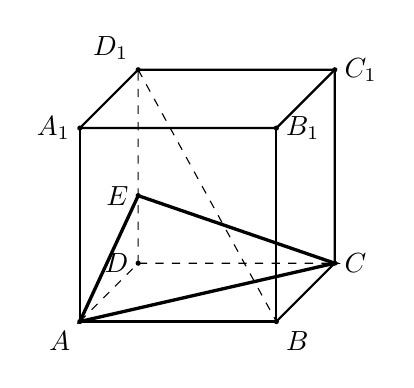
\begin{tikzpicture}[scale=0.78, >=stealth]
  \coordinate (A)  at (0,0);
  \coordinate (B)  at (3.2,0);
  \coordinate (C)  at (4.15,0.95);
  \coordinate (D)  at (0.95,0.95);
  \coordinate (A1) at (0,3.15);
  \coordinate (B1) at (3.2,3.15);
  \coordinate (C1) at (4.15,4.1);
  \coordinate (D1) at (0.95,4.1);
  \coordinate (E)  at (0.95,2.05);

  \draw[thick] (A)--(B)--(B1)--(A1)--cycle;
  \draw[thick] (A1)--(B1)--(C1)--(D1)--cycle;
  \draw[thick] (B)--(C)--(C1);
  \draw[dashed] (A)--(D)--(C) (D)--(D1) (A1)--(D1);
  \draw[dashed] (D1)--(B);
  \draw[very thick] (A)--(E)--(C)--cycle;

  \fill (A)  circle (1.2pt) node[below left] {$A$};
  \fill (B)  circle (1.2pt) node[below right] {$B$};
  \fill (C)  circle (1.2pt) node[right] {$C$};
  \fill (D)  circle (1.2pt) node[left] {$D$};
  \fill (A1) circle (1.2pt) node[left] {$A_1$};
  \fill (B1) circle (1.2pt) node[right] {$B_1$};
  \fill (C1) circle (1.2pt) node[right] {$C_1$};
  \fill (D1) circle (1.2pt) node[above left] {$D_1$};
  \fill (E)  circle (1.2pt) node[left] {$E$};
\end{tikzpicture}
\end{center}
\nopagebreak[4]
\Needspace{4\baselineskip}
\textbf{解析}

\Needspace{5\baselineskip}
建立直角坐标系：

\nopagebreak[4]
\[
A(0,0,0),\quad B(a,0,0),\quad C(a,a,0),\quad D(0,a,0),
\]

\Needspace{5\baselineskip}
并设正四棱柱的高为 $h$，令 $E=(0,a,e)$，其中 $e=DE$。则

\nopagebreak[4]
\[
A_1=(0,0,h),\qquad B_1=(a,0,h),\qquad D_1=(0,a,h).
\]

\Needspace{5\baselineskip}
平面 $EAC$ 的一个法向量可取

\nopagebreak[4]
\[
\mathbf n=(e,-e,a).
\]

\Needspace{5\baselineskip}
平面 $EAC$ 与底面所成角为 $45^\circ$，因此

\nopagebreak[4]
\[
\frac{a}{\sqrt{2e^2+a^2}}=\cos45^\circ=\frac1{\sqrt2},
\]

\Needspace{5\baselineskip}
得到

\nopagebreak[4]
\[
e=\frac a{\sqrt2}.
\]

\Needspace{5\baselineskip}
又因为 $D_1B$ 平行于平面 $EAC$，而

\nopagebreak[4]
\[
\overrightarrow{D_1B}=(a,-a,-h),
\]

\Needspace{5\baselineskip}
所以

\nopagebreak[4]
\[
\mathbf n\cdot\overrightarrow{D_1B}
=a^2(2e-h)=0,
\qquad h=2e=\sqrt2\,a.
\]

\gksubpart{(1)}

\Needspace{5\baselineskip}
由

\nopagebreak[4]
\[
\left|\overrightarrow{AC}\times\overrightarrow{AE}\right|
=a\sqrt{2e^2+a^2}=a^2\sqrt2,
\]

\Needspace{5\baselineskip}
得

\nopagebreak[4]
\[
S_{\triangle EAC}=\frac{a^2}{\sqrt2}.
\]

\gksubpart{(2)}

\Needspace{5\baselineskip}
直线 $A_1B_1$ 与 $AC$ 的方向向量分别可取 $(1,0,0)$、$(1,1,0)$，其公共垂线为竖直方向。该公共垂线在两直线上的端点为 $A_1$ 与 $A$，故距离为

\nopagebreak[4]
\[
A_1A=h=\sqrt2\,a.
\]

\gksubpart{(3)}

\Needspace{5\baselineskip}
平面 $EAC$ 的方程为

\nopagebreak[4]
\[
ex-ey+az=0.
\]

\Needspace{5\baselineskip}
点 $B_1$ 到该平面的距离为

\nopagebreak[4]
\[
\frac{ea+ah}{\sqrt{2e^2+a^2}}
=\frac{3a}{2}.
\]

\Needspace{5\baselineskip}
因此三棱锥 $B_1-EAC$ 的体积为

\nopagebreak[4]
\[
V=\frac13\cdot\frac{a^2}{\sqrt2}\cdot\frac{3a}{2}
=\frac{a^3}{2\sqrt2}.
\]

\gkanswer{答案（1）：$\dfrac{a^2}{\sqrt2}$}

\gkanswer{答案（2）：$\sqrt2\,a$}

\gkanswer{答案（3）：$\dfrac{a^3}{2\sqrt2}$}

\end{answer}
\begin{answer}
\gksolhead{22}{}

\textbf{题目}：

如图为一台冷轧机的示意图。冷轧机由若干对轧辊组成，带钢从一端输入，经过各对轧辊逐步减薄后输出。

\Needspace{5\baselineskip}
（1） 输入带钢的厚度为 $\alpha$，输出带钢的厚度为 $\beta$，若每对轧辊的减薄率不超过 $r_0$，问冷轧机至少需要安装多少对轧辊？

\nopagebreak[4]
\[
\text{\text{一对轧辊减薄率}}=\frac{\text{\text{输入该对的带钢厚度}}-\text{\text{从该对输出的带钢厚度}}}{\text{\text{输入该对的带钢厚度}}}。
\]

（2） 已知一台冷轧机共有 4 对减薄率为 20\\% 的轧辊，所有轧辊周长均为 1600。若第 $k$ 对轧辊有缺陷，每滚动一周在带钢上压出一个疵点，在冷轧机输出的带钢上，疵点的间距为 $L_k$。为了便于检修，请计算 $L_1$、$L_2$、$L_3$ 并填入下表（轧钢过程中，带钢宽度不变，且不考虑损耗）。

\begin{center}
\begin{tabular}{lrrrr}
\toprule
轧辊序号 & 1 & 2 & 3 & 4 \\
\midrule
疵点间距 $L_k$/mm &  &  &  & 1600 \\
\bottomrule
\end{tabular}
\end{center}
\nopagebreak[4]
\begin{center}% 1999 年全国卷理科第 22 题：冷轧机示意图
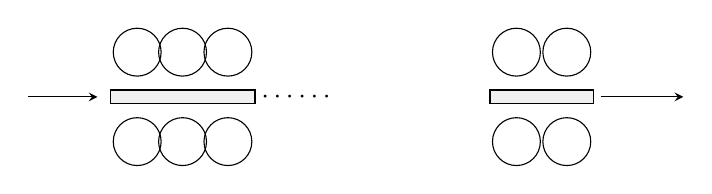
\begin{tikzpicture}[>=stealth, scale=0.8]
  \newcommand{\rollgroup}[2]{%
    \begin{scope}[xshift=#1cm]
      \draw[fill=gray!12] (-1.15,0.0) rectangle (1.15,0.22);
      \foreach \x in {-0.72,0,0.72} {
        \draw (\x,0.82) circle (0.38);
        \draw (\x,-0.60) circle (0.38);
      }
    \end{scope}%
  }
  \draw[->] (-6.15,0.11)--(-5.05,0.11);
  \rollgroup{-3.7}{}
  \node at (-1.9,0.1) {$\cdots\cdots$};
  \begin{scope}[xshift=2.0cm]
    \draw[fill=gray!12] (-0.82,0.0) rectangle (0.82,0.22);
    \foreach \x in {-0.4,0.4} {
      \draw (\x,0.82) circle (0.38);
      \draw (\x,-0.60) circle (0.38);
    }
  \end{scope}
  \draw[->] (2.95,0.11)--(4.25,0.11);
\end{tikzpicture}
\end{center}
\nopagebreak[4]
\Needspace{4\baselineskip}
\textbf{解析}

\gksubpart{(1)}

\Needspace{5\baselineskip}
设经过 $m$ 对轧辊后的厚度为 $t_m$。每对轧辊的减薄率不超过 $r_0$，所以

\nopagebreak[4]
\[
t_m\ge\alpha(1-r_0)^m.
\]

\Needspace{5\baselineskip}
要达到厚度 $\beta$，必须有

\nopagebreak[4]
\[
\alpha(1-r_0)^m\le\beta.
\]

\Needspace{5\baselineskip}
在 $0<r_0<1$、$0<\beta<\alpha$ 时，这等价于

\nopagebreak[4]
\[
m\ge\log_{1-r_0}\frac\beta\alpha.
\]

\Needspace{5\baselineskip}
故至少需要

\nopagebreak[4]
\[
m_{\min}
=\left\lceil\log_{1-r_0}\frac\beta\alpha\right\rceil
\]

对轧辊。

\gksubpart{(2)}

\Needspace{5\baselineskip}
每对轧辊的厚度缩小为原来的 $0.8$ 倍。第 $k$ 对轧辊产生的疵点，在该对轧辊之后的初始间距为 $1600\ \mathrm{mm}$；经过后面的轧辊，带钢长度按厚度反比伸长。因此

\nopagebreak[4]
\[
L_k=1600\frac{0.8^k}{0.8^4}
=\frac{1600}{0.8^{4-k}}\ \mathrm{mm}.
\]

\Needspace{5\baselineskip}
于是

\nopagebreak[4]
\[
L_1=3125\ \mathrm{mm},\qquad
L_2=2500\ \mathrm{mm},\qquad
L_3=2000\ \mathrm{mm}.
\]

\gkanswer{答案（1）：$\left\lceil\log_{1-r_0}\dfrac{\beta}{\alpha}\right\rceil$ 对轧辊（$0<\beta<\alpha$，$0<r_0<1$）。}

\gkanswer{答案（2）：$L_1=3125\ \mathrm{mm}$，$L_2=2500\ \mathrm{mm}$，$L_3=2000\ \mathrm{mm}$。}

\end{answer}
\begin{answer}
\gksolhead{23}{}

\textbf{题目}：

已知函数 $y=f(x)$ 的图象是自原点出发的一条折线，当 $n\le y\le n+1\ (n=0,1,2,\ldots)$ 时，该图象是斜率为 $b^n$ 的线段（其中正常数 $b\ne1$），设数列 $\{x_n\}$ 由 $f(x_n)=n\ (n=1,2,\ldots)$ 定义。

（1） 求 $x_1$、$x_2$ 和 $x_n$ 的表达式；

（2） 求 $f(x)$ 的表达式，并写出其定义域；

（3） 证明：$y=f(x)$ 的图象与 $y=x$ 的图象没有横坐标大于 1 的交点。

\Needspace{4\baselineskip}
\textbf{解析}

\gksubpart{(1)}

\Needspace{5\baselineskip}
设 $x_0=0$。第 $k$ 段的斜率为 $b^k$，纵坐标增加 $1$ 时横坐标增加 $b^{-k}$，所以

\nopagebreak[4]
\[
x_n=\sum_{k=0}^{n-1}b^{-k}.
\]

\Needspace{5\baselineskip}
从而

\nopagebreak[4]
\[
x_1=1,\qquad
x_2=1+\frac1b,
\qquad
x_n=\frac{1-b^{-n}}{1-b^{-1}}
=\frac b{b-1}\left(1-b^{-n}\right).
\]

\gksubpart{(2)}

\Needspace{5\baselineskip}
在区间 $x_n\le x\le x_{n+1}$ 上，图象所在的线段从 $(x_n,n)$ 连接到 $(x_{n+1},n+1)$，故

\nopagebreak[4]
\[
f(x)=n+b^n(x-x_n),
\qquad x_n\le x\le x_{n+1},
\quad n=0,1,2,\ldots.
\]

\Needspace{5\baselineskip}
当 $b>1$ 时，$x_n$ 的极限为 $\dfrac b{b-1}$，定义域为

\nopagebreak[4]
\[
\left[0,\frac b{b-1}\right);
\]

当 $0<b<1$ 时，$x_n\to+\infty$，定义域为 $[0,+\infty)$。

\gksubpart{(3)}

\Needspace{5\baselineskip}
最后证明第（3）问。若 $b>1$，则对 $n\ge1$ 有 $x_n\le n$，且除 $x_1=n=1$ 外为严格不等式。因此在每个 $x>1$ 的线段端点上均有 $f(x)-x>0$，而线段上 $f(x)-x$ 是一次函数，所以

\nopagebreak[4]
\[
f(x)>x\qquad(x>1).
\]

\Needspace{5\baselineskip}
若 $0<b<1$，则 $x_n\ge n$，且从 $x_2$ 起严格大于 $n$。在 $x=1$ 处两图象相交；其后每个线段端点均满足 $f(x)-x<0$，故

\nopagebreak[4]
\[
f(x)<x\qquad(x>1).
\]

两种情形都说明横坐标大于 $1$ 时没有交点。

\gkanswer{答案（1）：$x_1=1$，$x_2=1+\dfrac1b$，$x_n=\displaystyle\sum_{k=0}^{n-1}b^{-k}=\dfrac b{b-1}\left(1-b^{-n}\right)$。}

\gkanswer{答案（2）：$f(x)=n+b^n(x-x_n)$（$x_n\le x\le x_{n+1}$，$n=0,1,2,\ldots$）；$b>1$ 时定义域为 $\left[0,\dfrac b{b-1}\right)$，$0<b<1$ 时定义域为 $[0,+\infty)$。}

\gkanswer{答案（3）：$b>1$ 时 $x>1$ 有 $f(x)>x$，$0<b<1$ 时 $x>1$ 有 $f(x)<x$，所以没有横坐标大于 1 的交点。}

\end{answer}
\begin{answer}
\gksolhead{24}{}

\textbf{题目}：

如图，给出定点 $A(a,0)\ (a>0)$ 和直线 $l:x=-1$。$B$ 是直线 $l$ 上的动点，$\angle BOA$ 的角平分线交 $AB$ 于点 $C$。求点 $C$ 的轨迹方程，并讨论方程表示的曲线类型与 $a$ 值的关系。
\nopagebreak[4]
\begin{center}% 1999 年全国卷理科第 24 题：角平分线轨迹示意图
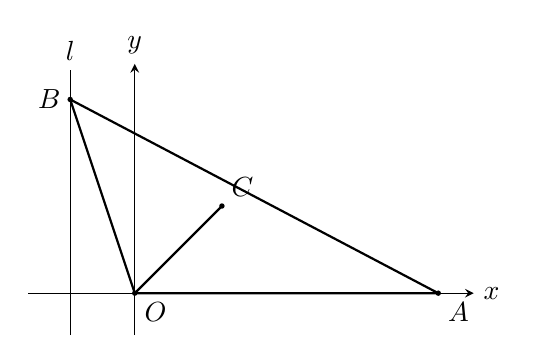
\begin{tikzpicture}[>=stealth, scale=0.82]
  \coordinate (O) at (0,0);
  \coordinate (A) at (4.7,0);
  \coordinate (B) at (-1,3.0);
  \coordinate (C) at (1.35,1.35);

  \draw[->] (-1.65,0)--(5.25,0) node[right] {$x$};
  \draw[->] (0,-0.65)--(0,3.55) node[above] {$y$};
  \draw (-1,-0.65)--(-1,3.45) node[above] {$l$};
  \draw[thick] (B)--(A);
  \draw[thick] (B)--(O)--(A);
  \draw[thick] (O)--(C);

  \fill (O) circle (1.2pt) node[below right] {$O$};
  \fill (A) circle (1.2pt) node[below right] {$A$};
  \fill (B) circle (1.2pt) node[left] {$B$};
  \fill (C) circle (1.2pt) node[above right] {$C$};
\end{tikzpicture}
\end{center}
\nopagebreak[4]
\Needspace{4\baselineskip}
\textbf{解析}

\Needspace{5\baselineskip}
令动点 $B=(-1,u)$，记

\nopagebreak[4]
\[
r=OB=\sqrt{1+u^2}.
\]

\Needspace{5\baselineskip}
在三角形 $OAB$ 中，由角平分线定理

\nopagebreak[4]
\[
\frac{AC}{CB}=\frac{OA}{OB}=\frac ar.
\]

\Needspace{5\baselineskip}
于是点 $C$ 的坐标为

\nopagebreak[4]
\[
x=\frac{ar-a}{a+r}
=\frac{a(r-1)}{a+r},
\qquad
y=\frac{au}{a+r}.
\]

\Needspace{5\baselineskip}
由第一式可得

\nopagebreak[4]
\[
r=\frac{a(x+1)}{a-x},
\]

\Needspace{5\baselineskip}
再由第二式得到

\nopagebreak[4]
\[
u=\frac{(a+1)y}{a-x}.
\]

\Needspace{5\baselineskip}
代入 $r^2-u^2=1$，有

\nopagebreak[4]
\[
a^2(x+1)^2-(a+1)^2y^2=(a-x)^2.
\]

\Needspace{5\baselineskip}
化简得轨迹方程

\nopagebreak[4]
\[
(a-1)x^2+2ax-(a+1)y^2=0.
\]

由参数表达式还可知实际轨迹满足 $0\le x<a$；上式是其所在二次曲线的方程。分类如下：

\begin{itemize}
\item $a>1$ 时，$x^2$ 与 $y^2$ 的系数异号，表示双曲线；
\item $a=1$ 时，方程为 $x=y^2$，表示抛物线；
\item $0<a<1$ 时，整理为
\end{itemize}
\nopagebreak[4]
  \[
  (1-a)x^2+(a+1)y^2=2ax,
  \]
  表示椭圆。

\gkanswer{答案：轨迹方程为 $(a-1)x^2+2ax-(a+1)y^2=0$；$a>1$ 时为双曲线，$a=1$ 时为抛物线 $x=y^2$，$0<a<1$ 时为椭圆。}

\end{answer}
\begin{answer}
\gksolhead{25}{}

\textbf{题目}：

已知数列 $\{b_n\}$ 是等差数列，$b_1=1$，$b_1+b_2+\cdots+b_{10}=145$。

（1） 求数列 $\{b_n\}$ 的通项 $b_n$；

\Needspace{5\baselineskip}
（2） 设数列 $\{a_n\}$ 的通项

\nopagebreak[4]
\[
a_n=\log_a\left(1+\frac1{b_n}\right)
\]

（其中 $a>0$，且 $a\ne1$），记 $S_n$ 是数列 $\{a_n\}$ 的前 $n$ 项和。试比较 $S_n$ 与 $\dfrac13\log_a b_{n+1}$ 的大小，并证明你的结论。

\Needspace{4\baselineskip}
\textbf{解析}

\gksubpart{(1)}

\Needspace{5\baselineskip}
设等差数列 $\{b_n\}$ 的公差为 $d$。由

\nopagebreak[4]
\[
145=S_{10}=\frac{10(2b_1+9d)}2
=5(2+9d),
\]

\Needspace{5\baselineskip}
得到 $d=3$，所以

\nopagebreak[4]
\[
b_n=1+3(n-1)=3n-2.
\]

\gksubpart{(2)}

\Needspace{5\baselineskip}
由于 $b_n=3n-2>0$，

\nopagebreak[4]
\[
a_n=\log_a\left(\frac{b_n+1}{b_n}\right)
=\log_a\frac{3n-1}{3n-2}.
\]

\Needspace{5\baselineskip}
令

\nopagebreak[4]
\[
P_n=\prod_{k=1}^n\frac{3k-1}{3k-2},
\]

\Needspace{5\baselineskip}
则

\nopagebreak[4]
\[
S_n=\log_a P_n.
\]

\Needspace{5\baselineskip}
对每个 $k\ge1$，令 $m=3k-1$，有

\nopagebreak[4]
\[
m^3-(m-1)^2(m+2)=3m-2>0.
\]

\Needspace{5\baselineskip}
即

\nopagebreak[4]
\[
\left(\frac{3k-1}{3k-2}\right)^3
>\frac{3k+1}{3k-2}.
\]

\Needspace{5\baselineskip}
相乘并利用连乘的望远镜关系，得到

\nopagebreak[4]
\[
P_n^3
>
\prod_{k=1}^n\frac{3k+1}{3k-2}
=\frac{3n+1}{1}
=b_{n+1}.
\]

\Needspace{5\baselineskip}
所以

\nopagebreak[4]
\[
P_n>b_{n+1}^{1/3}.
\]

\Needspace{5\baselineskip}
当 $a>1$ 时对数函数递增，故

\nopagebreak[4]
\[
S_n=\log_aP_n
>\frac13\log_ab_{n+1}.
\]

\Needspace{5\baselineskip}
当 $0<a<1$ 时对数函数递减，不等号反向，故

\nopagebreak[4]
\[
S_n<\frac13\log_ab_{n+1}.
\]

\gkanswer{答案（1）：$b_n=3n-2$}

\gkanswer{答案（2）：$a>1$ 时 $S_n>\dfrac13\log_a b_{n+1}$；$0<a<1$ 时 $S_n<\dfrac13\log_a b_{n+1}$。}

\end{answer}